\chapter{Introduzione}
\section{Obiettivo}
Lo scopo del presente progetto è la creazione di un'applicazione desktop per la gestione di password. Il programma offre le seguenti features:
\begin{itemize}
	\item Salvataggio dei dati su un Database NoSQL Mongo
	\item Interfaccia grafica sia per il login al programma che per la gestione delle password
	\item Avviso in caso di presenza di password scadute
	\item Possibilità di ricerca tramite parte del sito o dell'utenza
	\item Vista di riepilogo di tutte le password e possibilità di ordinamento in base a sito, utente, password o data di scadenza
	\item Gestione multi-utente per consentire l'utilizzo a diverse persone sullo stesso PC mantenendo i dati separati
\end{itemize}
\newpage
\section{Strumenti utilizzati}
Per lo sviluppo e il test del progetto sono stati usati i seguenti strumenti:
\begin{itemize}
	\item[\tool{Maven}] Consente di gestire le dipendenze e la build automation del progetto.

	\item[\tool{Travis}] Consente di avere una CI (Continuous Integration) gestita in maniera semplice attraverso il file di configurazione. Ad ogni push sul repository Git viene eseguita una build completa. Al termine viene inviato il riepilogo della code coverage a Coveralls e il riepilogo della code quality a Sonarcloud.

	\item[\tool{Coveralls}] Consente di consultare in maniera semplice il riepilogo della code coverage avendo sempre sotto controllo eventuali porzioni di codice non testate.

	\item[\tool{Sonar}] Consente di analizzare la qualità del codice segnalando tutte le anomalie riscontrate con la corrispettiva severity e il tempo di ``debito'' accumulato.

	\item[\tool{Docker}] Consente di usare dei contenitori all'interno dei quali è possibile eseguire server, database, singole applicazioni, sistemi operativi, ...

	\item[\tool{PIT}] Consente di verificare la completezza dei test preparati. Questo tool infatti genera una serie di mutazioni al codice delle classi del progetto che vengono quindi sottoposte ai test preparati. Eventuali mutazioni ``sopravvissute'' ai test vengono segnalate poiché indicano una probabile incompletezza nei test.

	\item[\tool{SWTBot}] È un tool per il test di interfacce grafiche basate su SWT, Eclipse o GEF (Graphical Editing Framework). Consente durante i test di simulare il comportamento di un utente che interagisce con l'interfaccia: fa click sui pulsanti, scrive nei campi editabili, vede cosa è presente nella finestra, ...
	
	\item[\tool{Fongo}] Il programma utilizza il Database Mongo come server per il salvataggio dei dati. Per evitare di dover mockare tutti i metodi delle API Java di Mongo, negli Unit Test è stato utilizzato \tool{Fongo} che consente di simulare il server Mongo mettendo a disposizione praticamente tutte le medesime funzionalità.
\end{itemize}

\chapter{Implementazione}
In questo capitolo sarà esposta la struttura del progetto che, come si vede dall'immagine, è composta da due folder distinte: \textit{src/main/java} per le classi che compongono il programma e \textit{src/test/java} per le classi di unit/integration test.
\begin{center}
	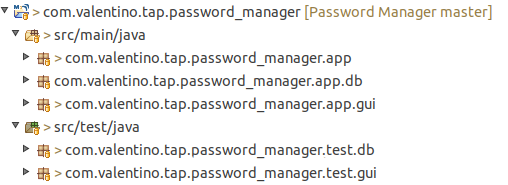
\includegraphics[width=15cm]{Immagini/Struttura.png}
\end{center}
\newpage
\section{Folder Main}
Il progetto è diviso in 3 package differenti: \emph{app}, \emph{app.db} e \emph{app.gui}.
\subsection{Package app}
Questo package gestisce la parte generale dell'applicazione. Qui sono contenute 3 classi:
\begin{myitemize}{\class{PasswordManager}}
	\item[\class{Password}] Questa classe modella l'oggetto password (composta da sito, utente, password e data di scadenza) e ne contiene i relativi metodi getter/setter.
		\begin{center} 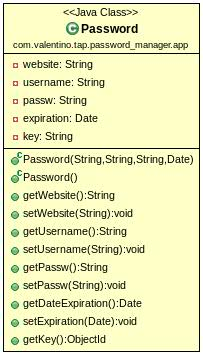
\includegraphics[width=6cm]{Immagini/Password.jpg} \end{center}
	\item[\class{PasswordManager}] Questa classe contiene le funzionalità per la gestione delle password: aggiunta, aggiornamento, cancellazione, verifica esistenza e ricerca tramite parte del sito o dell'utenza.
		\begin{center} 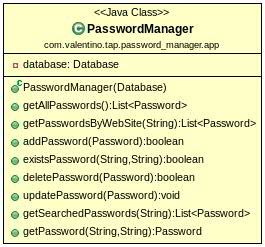
\includegraphics[width=6cm]{Immagini/PasswordManager.jpg} \end{center}		
	
	\item[\class{Application}] Questa classe contiene semplicemente il metodo principale dell'applicazione: mostra la finestra di accesso e, una volta effettuato il login/registrazione, mostra la finestra per la gestione delle password presenti per l'utente.
\end{myitemize}

\subsection{Package app.db}
In questo package sono presenti le classi per la gestione dell'interazione con il Database.
\begin{myitemize}{\class{MongoDatabaseWrapper}}
	\item[\class{Database}] Questa interfaccia contiene la definizione di tutti i metodi richiamati per interagire con il database. Avendo definito un'interfaccia è molto più semplice l'aggiunta di nuove tipologie di database con cui interagire: sarà sufficiente creare una nuova classe che implementi tale interfaccia.

	\item[\class{MongoDatabaseWrapper}] Questa classe è attualmente l'unica implementazione dell'interfaccia \class{Database} e contiene tutti i metodi per l'interazione con il database NoSQL Mongo. Viene utilizzata nel progetto sia per la gestione dell'accesso iniziale aprendo una connessione al database \emph{admin} (per recuperare l'elenco degli utenti presenti e registrare eventuali nuovi utenti), sia per la gestione delle password aprendo una connessione al database relativo all'utente loggato.
		\begin{center} 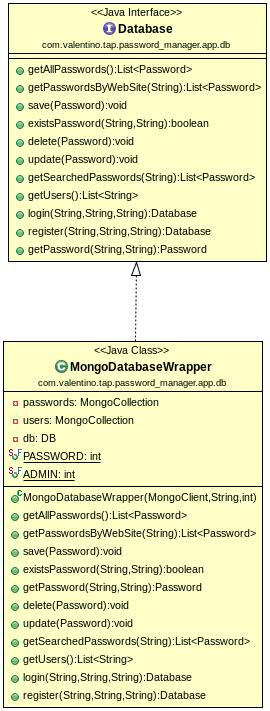
\includegraphics[height=15cm]{Immagini/DB.jpg} \end{center}
	
	\item[\class{DBUser}] Questa classe modella l'utente del database Mongo per consentire la gestione del login (recuperando l'elenco degli utenti esistenti) e la registrazione di nuovi utenti.
\end{myitemize}	
\newpage
\subsection{Package app.gui}
In questo package sono presenti le classi per la gestione dell'interfaccia grafica e di tutte le funzionalità collegate.
\begin{myitemize}{\class{PasswordManagerGUI}}
	\item[\class{LoginGUI}] Mostra la finetra iniziale per il login di utenti registrati o la registrazione di nuovi utenti.
		\begin{center} 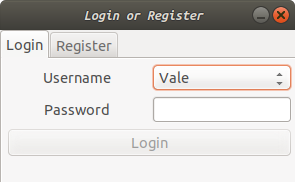
\includegraphics[width=6cm]{Immagini/Login.png} 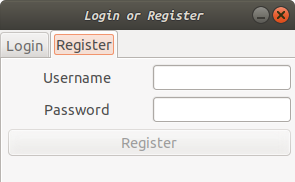
\includegraphics[width=6cm]{Immagini/Register.png}  \end{center}
		
	\item[\class{PasswordManagerGUI}] Contiene l'interfaccia principale per la gestione delle password: i pulsanti con le varie funzionalità, la barra di ricerca e la tabella con l'elenco delle password salvate in cui si può modificare l'ordinamento con un click sulla colonna secondo cui si vuole effettuare l'ordinamento.
		\begin{center} 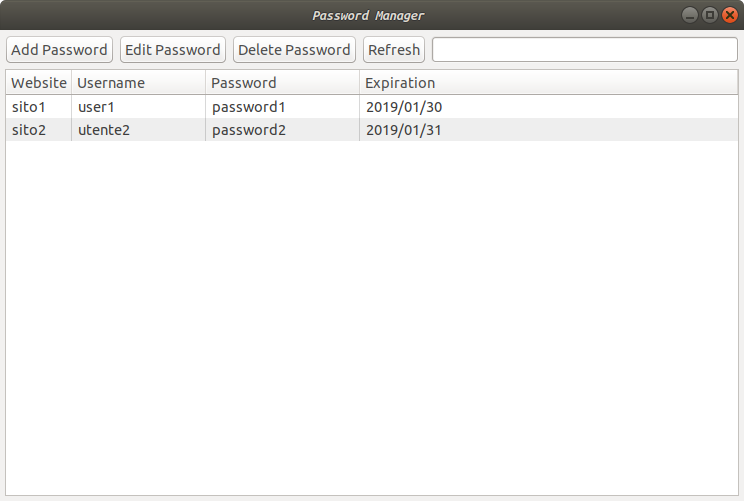
\includegraphics[width=12cm]{Immagini/PasswordGUI.png} \end{center}		

	\item[\class{EditDialog}] In questa classe è presente la finestra che viene mostrata per la creazione di una nuova password o per la modifica di una password esistente.
		\begin{center}
		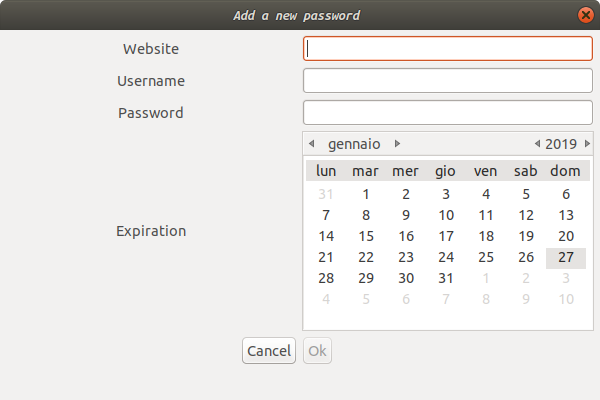
\includegraphics[width=12cm]{Immagini/AddGUI.png}
		\end{center}
				\begin{center}
		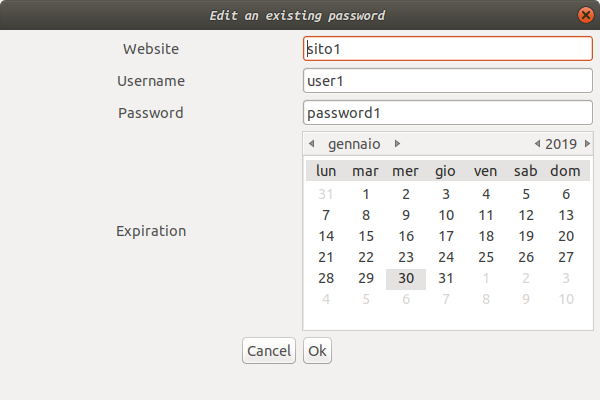
\includegraphics[width=12cm]{Immagini/EditGUI.png}
		\end{center}
		
	\item[\class{MessageDialog}] Inizialmente per la gestione dei messaggi di avviso o errore era stata usata la classe \class{org.eclipse.swt.widgets.MessageBox} ma, visto che tale classe non era testabile con \tool{SWTBot} a causa di un \link{https://bugs.eclipse.org/bugs/show_bug.cgi?id=164192}{bug aperto}, è stata implementata una classe custom.

	\item[\class{Labels}] Questa classe contiene le ``costanti'' per la parte grafica: label, hint, titoli, \\ messaggi, ... In questo modo è possibile richiamare lo stesso testo in diversi punti del programma in maniera sempre consistente evitando eventuali disallineamenti che potrebbero nascere dalla ridondanza.
\end{myitemize}

\section{Folder Test}
La cartella contenente i test è composta da due package: \emph{test.gui} e \emph{test.db}.
\subsection{Package test.gui}
In questo package sono presenti le classi per il test dell'interfaccia grafica. Per tali test è stato utilizzato il tool \tool{SWTBot} menzionato nel capitolo precedente.
\begin{myitemize}{\class{PasswordManagerGUITest}}
	\item[\class{LoginGUITestIT}] Verifica che sia correttamente mostrata la finestra con i tutti gli elementi attesi ed effettua i test per quanto riguarda l'accesso al progamma: si testa il login con le corrette credenziali, il mancato accesso con credenziali errate, la corretta registrazione di un nuovo utente e la mancata registrazione in caso di utente omonimo già presente. Viene inoltre verificato che dopo aver effettuato l'accesso con successo (sia tramite login che tramite registrazione di un nuovo utente), venga correttamente mostrata la finestra principale del programma.
	
	\item[\class{PasswordManagerGUITest}] Verifica che sia correttamente mostrata la finestra con tutti gli elementi attesi e ne testa tutte le funzionalità. Si verifica inoltre che in caso di comportamento errato da parte dell'utente vengano mostrati i corretti messaggi d'errore: per esempio se si tenta di inserire due password per lo stesso sito/utenza o si tenta di inserire una password con data di scadenza errata.
\end{myitemize}
\newpage
\subsection{Package test.db}
In questo package troviamo i test principali sulle funzionalità backend del programma e sull'interazione con il database. Sono stati implementati sia degli unit test che degli integration test. Alcuni test effettuati nelle varie classi risultano però molto simili o identici, per tale motivo in seguito ad alcuni refactoring, tutti i test comuni sono stati raggruppati in classi astratte. Prima di procedere vediamo quindi le dipendenze tra le varie classi appartenenti a tale package riportate in figura \ref{fig:strutturaTest} a pagina \pageref{fig:strutturaTest}.
\begin{figure}[h]
		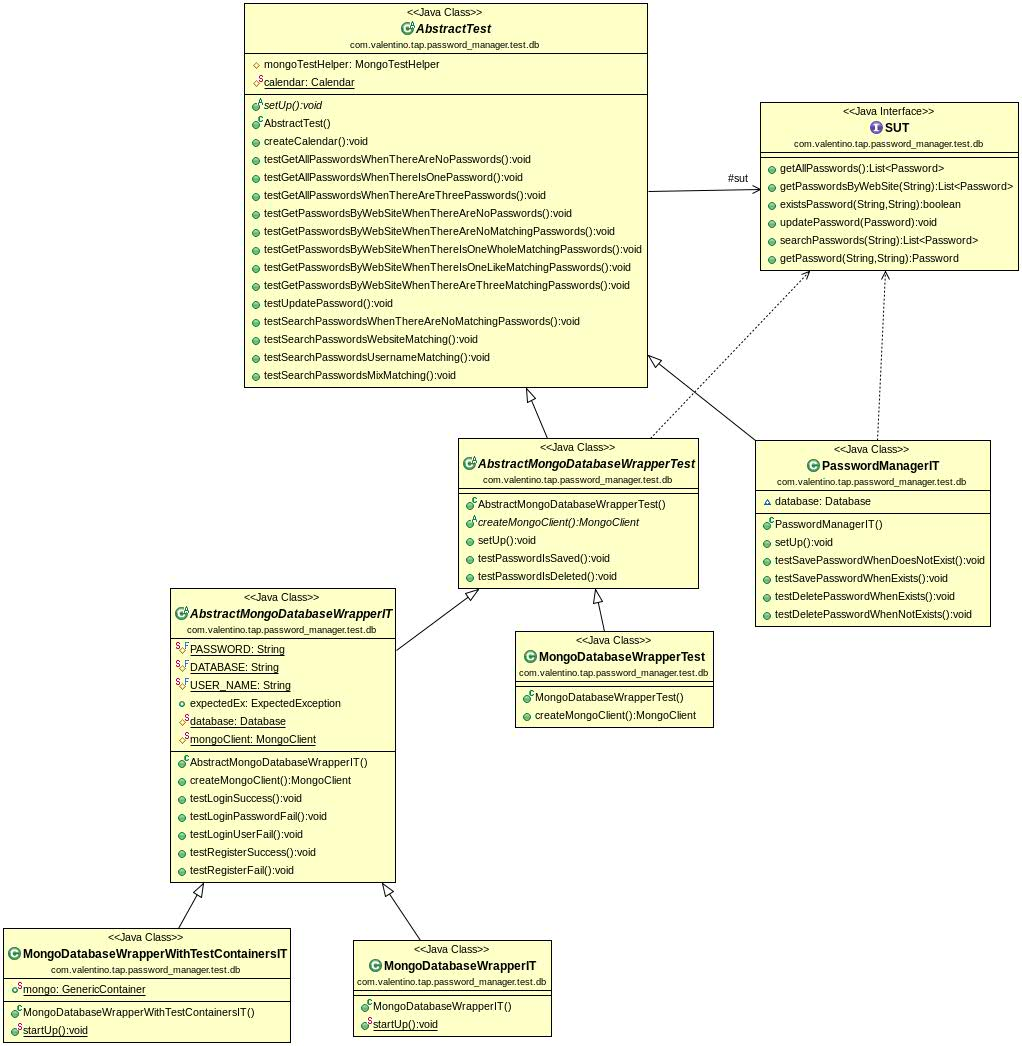
\includegraphics[scale=0.5]{Immagini/StrutturaTest.jpg}
	\caption{Struttura classi package test.db}
	\label{fig:strutturaTest}
\end{figure}
Come possiamo notare la classe in cui è presente la maggior implementazione è \class{AbstractTest}. In ogni test si fa riferimento all'interfaccia \class{SUT} che rappresenta appunto il \emph{Software Under Test}, in questo modo i test sono generici e indipendenti dalla classe che stiamo testando. Tale interfaccia è implementata dalle due classi \class{PasswordManagerTester} e \class{MongoTester}: la prima implementa le funzionalità necessarie richiamando i corrispettivi metodi della classe \class{PasswordManager}, la seconda i metodi della classe \class{MongoDatabaseWrapper}.
	\begin{center}
		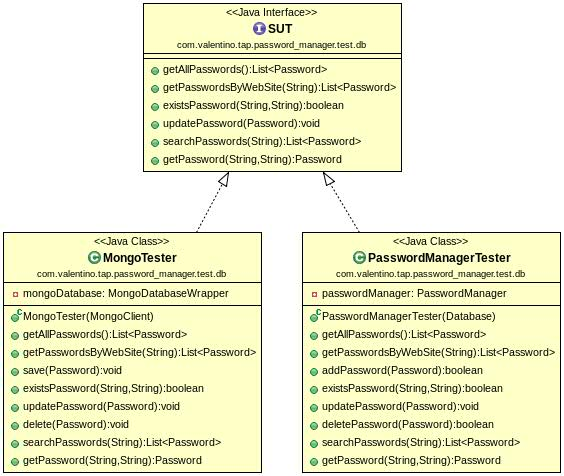
\includegraphics[width=10cm]{Immagini/SUT.jpg}
	\end{center}

Il metodo \test{testUpdatePassword}, per esempio, sarà richiamato sia durante i test della classe \class{PasswordManagerIT} che durante i test delle classi che estendono la classe astratta \class{AbstractMongoDatabaseWrapperTest}: nel primo caso verificherà il corretto aggiornamento della password quando viene richiesto dalla classe \class{PasswordManager}, nel secondo caso quando viene richiesto dalla classe \class{MongoDatabaseWrapper}. Centralizzando i test nella classe astratta è stato quindi possibile ridurre la quantità di codice scritta per i medesimi test e semplificare la scrittura di successivi test ad ogni aggiunta di nuove funzionalità.

Per quanto riguarda la classe \class{MongoDatabaseWrapper} sono stati implementati sia Unit test che Integration Test, infatti la classe astratta \class{AbstractMongoDatabaseWrapperTest} è estesa dalla classe \class{MongoDatabaseWrapperTest} (Unit Test) e dalla classe \\ \class{AbstractMongoDatabaseWrapperIT} (Integration Test). Si può notare che anche quest'ultima è una classe astratta poiché gli stessi Integration Test (principalmente per scopo didattico) sono eseguiti due volte: per quanto riguarda la classe \class{MongoDatabaseWrapperIT} connettendosi a un'istanza \tool{Mongo} presente in un docker avviato da \tool{Maven}, per quanto riguarda la classe \class{MongoDatabaseWrapperWithTestContainersIT} lanciando un apposito docker con l'istanza di \tool{Mongo}. Nella classe \class{AbstractMongoDatabaseWrapperIT} sono presenti i test sulle funzionalità di \class{MongoDatabaseWrapper} per quanto riguarda la gestione degli accessi: login, registrazione nuovi utenti, verifica utenti presenti, ... Tali test infatti, con lo stesso principio visto in precedenza, vengono quindi eseguiti sia sul docker lanciato da \tool{Maven} che sul docker lanciato dalla classe \class{MongoDatabaseWrapperWithTestContainersIT}.
Per concludere quindi possiamo osservare che le classi \class{MongoDatabaseWrapperTest}, \class{MongoDatabaseWrapperIT} e \class{MongoDatabaseWrapperWithTestContainersIT} contengono solo una differente creazione del MongoClient che viene utilizzato per i test.

\chapter{Difficoltà riscontrate}
Di seguito sono esposte le principali difficoltà incontrate:
\begin{itemize}
	\item Inizialmente non era molto naturale la scrittura e l'esecuzione dei test prima dell'implementazione stessa ma risultava quasi una forzatura. Dopo non molto però si sono visti i vantaggi sia in termini di velocità di sviluppo (anche grazie alle molteplici funzionalità offerte da Eclipse) sia in termini di correttezza di design e modello.
	\item Altra difficoltà è stata l'utilizzo del Database Mongo per la gestione degli utenti e degli accessi. Pur avendo buona padronanza (per lavoro) di SQL e PL/SQL su Oracle ho avuto qualche difficoltà a orientarmi e comprendere l'organizzazione del database Mongo, la creazione degli utenti con i relativi  permessi e il recupero degli utenti esistenti.
	\item Le password scadute vengono evienziate dal programma tramite il colore rosso nel riepilogo principale e tramite una pop-up con il relativo messaggio come possiamo vedere dalle seguenti immagini. 
	\begin{center}
		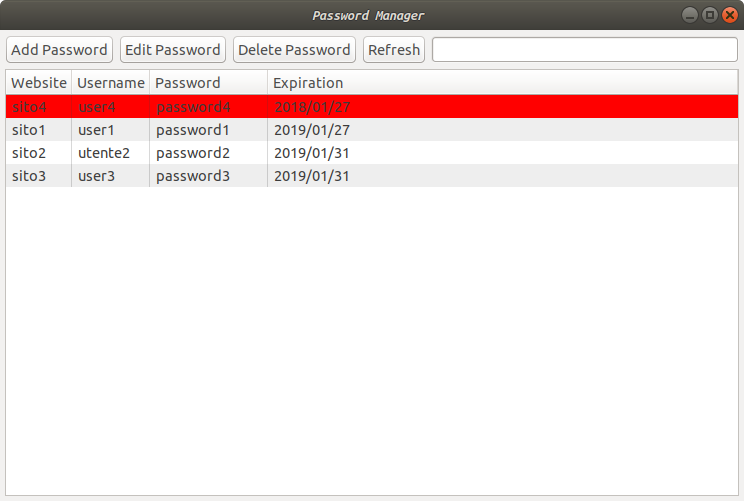
\includegraphics[width=12cm]{Immagini/Expired.png}
		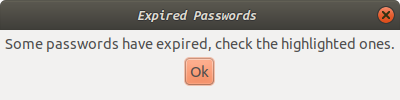
\includegraphics[width=8cm]{Immagini/ExpiredMsg.png}	
	\end{center}
	Non è stato però possibile testare la corretta colorazione delle righe relative alle password scadute con \tool{SWTBot} in quanto gli elementi delle tabelle non vengono gestiti, a differenza di altri Widget, come istanze della classe \class{org.eclipse.swt.widgets.Control}, di conseguenza non viene correttamente recuperato da \tool{SWTBot} il colore. Per tale motivo i test relativi al colore delle righe della tabella all'interno della classe \class{PassworManagerGUI} sono stati commentati ed è stato riportato il riferimento alla \link{https://www.eclipse.org/forums/index.php/m/485822/}{nota}.
	\item Infine, anche se abbastanza normale, altre difficoltà sono nate dall'utilizzo di strumenti nuovi da dover imparare. Inizialmente per esempio ho perso diverso tempo per l'aggiunta di \tool{SWTBot} alle dipendenze visto che non è presente su \emph{Maven Central} o per comprendere l'organizzazione e la gestione del file \emph{pom}.
\end{itemize}

\chapter{Dettagli}
Il progetto è presente su \link{https://github.com/valentino-marano/Password-Manager}{Github}, nel file \emph{README} sono presenti anche i badge con i collegamenti verso \link{https://travis-ci.org/valentino-marano/Password-Manager}{Travis}, \link{https://coveralls.io/github/valentino-marano/Password-Manager?branch=master}{Coveralls} e \link{https://sonarcloud.io/dashboard?id=com.valentino.tap\%3Apassword_manager}{Sonarcloud}. 

\noindent
È possibile effettuare la build anche da terminale usando il comando 
\begin{minted}[breaklines]{bash}
mvn -f com.valentino.tap.password_manager/pom.xml clean verify -Pjacoco coveralls:report sonar:sonar
\end{minted}
In questo modo saranno sarà effettuata la build con tutti i test; avendo attivato l'apposito profilo sarà inoltre effettuata la code coverage tramite \tool{JaCoCo} e il report sarà inviato a \tool{Coveralls}. Al termine della build, l'applicazione viene inclusa in un apposito contenitore ed è stato aggiunto un docker-compose file per gestire l'avvio sia del docker con l'applicazione che del docker con l'istanza di \tool{Mongo} necessaria. Per l'avvio di tali docker è stato predisposto lo script \emph{password\_manager.sh}. 

\noindent
Da riga di comando è inoltre possibile effettuare i mutation test con il comando
\begin{minted}[breaklines]{bash}
mvn -f com.valentino.tap.password_manager/pom.xml docker:start org.pitest:pitest-maven:mutationCoverage docker:stop
\end{minted}
Questo consente l'avvio del docker con \tool{Mongo} prima dei mutation test e la chiusura di tale docker al termine. 

\chapter{Possibili Estensioni}
Elenchiamo di seguito alcune delle possibili estensioni:
\begin{itemize}
	\item Sviluppo di un'app per smartphone sincronizzabile con il software presente sul PC.
	\item Possibilità di sincronizzare le password su un server in modo da avere sempre un backup.
	\item Possibilità di importare/esportare il contenuto del Database tramite dump protetto.
	\item Possibilità di testare la robustezza delle proprie password con appositi tool che effettuano attachi brute force, attacchi al dizionario o simili.
	\item Possibilità di generare password randomiche impostando alcuni parametri (es. lunghezza massima, caratteri speciali, ...)
	\item Aggiunta del pulsante che copia la password automaticamente in modo da averla subito a disposizione per incollarla senza doverla selezionare.
\end{itemize}